

Considering that stability is a crucial feature of benchmarking, in this paper, we specifically design a virtual API server and stable evaluation system to improve the stability based on ToolBench, and propose a new benchmark, named StableToolBench.

\subsection{Virtual API Server}

With real APIs, many of the failures encountered when reproducing its experiments are caused by expired APIs, network issues, or failed authentication.
To address this problem, we specifically propose a virtual API server with two components as illustrated in~\Cref{fig:main_figure}, including a caching system and API simulator.
Moreover, we design API calling rules to combine these two components to ensure the virtual API server is stable.



\paragraph{Caching System.}

We first implement a caching system that stores responses of all API callings to ensure consistency.
The caching system uses keys composed of their category, tool, API name, and arguments.
As a start, we populate the initial cache using the API call history from the training data and the reproduced test data released in ToolBench\footnote{\url{https://drive.google.com/drive/folders/1yBUQ732mPu-KclJnuQELEhtKakdXFc3J}}.
% We also update the cache with the reproduced test data released in ToolBench.
% New responses will be continuously recorded when running the experiment.
To ensure the quality of cached APIs, only valid records following the rule in \Cref{app:filter_rule} will be saved.
It is worth noting that we will also reserve some APIs with exceptions to keep the reality.
In this way, most API responses will be readily available, allowing the benchmark focus on probing the tool usage ability of designed methods with minimal impact on tool availability.
Furthermore, the API call in new experiments will also be continuously updated in the cache to ensure scalability.
The statistics of cache are shown in \Cref{tab:cache_components}.
\begin{table}[h!]
    \centering
    \small
    \begin{tabular}{lcccc}
        \toprule
         \textbf{Source} & \textbf{Train Set} & \textbf{Test Set} & \textbf{New Exp} & \textbf{Total} \\
         \midrule
         \textbf{Before} & 58,105 & 5,921 & 255,828 & 352,630 \\
         \textbf{After} & 25,995 & 2,393 & 136,592 & 164,980 \\
         \bottomrule
    \end{tabular}
    \caption{Cache components and their sizes before and after filtration. The cache of new experiments is updated until 12 Feb 2024.}
    \label{tab:cache_components}
\end{table}
Additionally, as an extra benefit, this approach reduces the latency introduced by interacting with real APIs, and also saves the costs for the API simulator discussed below.
% The caching system ultimately accumulates a total of 164,980 items, comprising 25,995 items sourced from training data, 5,921 items derived from testing data, with the remainder originating from our collection and various experimental runs.

%  \begin{table*}[t!]
%     \centering
%     \small
%     \resizebox{\textwidth}{!}{
%     \begin{tabular}{lccccccc}
%         \toprule
%         \textbf{Method} & \textbf{I1 Instruction} & \textbf{I1 Category} & \textbf{I1 Tool} & \textbf{I2 Category} & \textbf{I2 Instruction} & \textbf{I3 Instruction} & \textbf{Average} \\
%         \midrule

%     3.5 0613 (C) & 55.9{\tiny $\pm{1.0}$} & 50.8{\tiny $\pm{0.8}$} & 55.9{\tiny $\pm{1.0}$} & 44.1{\tiny $\pm{0.8}$} & 36.2{\tiny $\pm{0.4}$} & 51.4{\tiny $\pm{1.5}$} & 49.1{\tiny $\pm{1.0}$} \\
%     3.5 0613 (D) & 66.4{\tiny $\pm{1.5}$} & 64.3{\tiny $\pm{1.0}$} & 67.2{\tiny $\pm{2.4}$} & 67.7{\tiny $\pm{0.8}$} & 61.5{\tiny $\pm{1.0}$} & 81.4{\tiny $\pm{1.5}$} & 68.1{\tiny $\pm{1.4}$} \\
%     4 0613 (C) & 50.7{\tiny $\pm{0.4}$} & 57.1{\tiny $\pm{0.3}$} & 51.9{\tiny $\pm{0.3}$} & 55.0{\tiny $\pm{1.1}$} & 61.6{\tiny $\pm{0.8}$} & 56.3{\tiny $\pm{0.8}$} & 55.4{\tiny $\pm{0.6}$} \\
%     4 0613 (D) & 65.5{\tiny $\pm{1.1}$} & 62.0{\tiny $\pm{1.7}$} & 72.1{\tiny $\pm{1.6}$} & \textbf{70.8}{\tiny $\pm{1.3}$} & \textbf{73.1}{\tiny $\pm{1.4}$} & 74.9{\tiny $\pm{1.5}$} & 69.7{\tiny $\pm{1.4}$} \\
%     T-LLaMA (C) & 37.2{\tiny $\pm{0.1}$} & 42.3{\tiny $\pm{0.4}$} & 43.0{\tiny $\pm{0.5}$} & 37.4{\tiny $\pm{0.4}$} & 33.6{\tiny $\pm{1.2}$} & 39.6{\tiny $\pm{1.0}$} & 38.9{\tiny $\pm{0.6}$} \\
%     T-LLaMA (D) & 59.8{\tiny $\pm{1.5}$} & 59.5{\tiny $\pm{1.4}$} & 65.7{\tiny $\pm{1.1}$} & 56.5{\tiny $\pm{0.3}$} & 47.6{\tiny $\pm{0.4}$} & 62.8{\tiny $\pm{1.9}$} & 58.7{\tiny $\pm{1.1}$} \\
%     \midrule
%     3.5 1106 (C) & 51.3{\tiny $\pm{0.6}$} & 48.8{\tiny $\pm{0.3}$} & 59.9{\tiny $\pm{0.8}$} & 50.8{\tiny $\pm{0.7}$} & 43.2{\tiny $\pm{0.8}$} & 58.5{\tiny $\pm{0.8}$} & 52.1{\tiny $\pm{0.7}$} \\
%     3.5 1106 (D) & 67.8{\tiny $\pm{0.9}$} & 67.2{\tiny $\pm{0.3}$} & \textbf{72.9}{\tiny $\pm{0.7}$} & 63.2{\tiny $\pm{1.0}$} & 70.9{\tiny $\pm{0.4}$} & 77.6{\tiny $\pm{0.8}$} & 69.9{\tiny $\pm{0.7}$} \\
%     4 Turbo (C) & 63.1{\tiny $\pm{1.0}$} & 64.5{\tiny $\pm{0.5}$} & 55.3{\tiny $\pm{0.3}$} & 63.0{\tiny $\pm{0.8}$} & 57.3{\tiny $\pm{0.8}$} & 61.7{\tiny $\pm{0.8}$} & 60.8{\tiny $\pm{0.7}$} \\
%     4 Turbo (D) & \textbf{70.8}{\tiny $\pm{1.0}$} & \textbf{71.1}{\tiny $\pm{0.7}$} & 70.4{\tiny $\pm{1.2}$} & 70.4{\tiny $\pm{1.3}$} & 71.7{\tiny $\pm{0.4}$} & \textbf{84.7}{\tiny $\pm{1.7}$} & \textbf{73.2}{\tiny $\pm{1.1}$} \\

%          \bottomrule
%     \end{tabular}
%     }
%     \caption{Solvable pass rate scores. We run all models once, evaluate three times and take the average results. ``3.5 0613'', ``4 0613'', ``3.5 1106'', ``4 Trubo'', ``T-LLaMA'' stands for \texttt{gpt-3.5-turbo-0613}, \texttt{gpt-4-0613}, \texttt{gpt-3.5-turbo-1106}, \texttt{gpt-4-turbo-preview}, 
%     \texttt{ToolLLaMA v2} respectively. C and D stand for CoT and DFS respectively. The experiments below follow the denotation.}
%     \label{tab:main_sopr}
% \end{table*}


\paragraph{API Simulator.}
Due to the limited coverage of the caching system, we propose to use LLMs to simulate API responses that are not in the cache and unavailable. 
Specifically, we ask \texttt{gpt-4-turbo} to simulate the API behaviour based on the original documentation in ToolBench.
The API documentation includes the descriptions of the functions and their corresponding parameters. 
% incorporate the documentation in the prompt of GPT-4 to generate a response given a requested input.
To mitigate the difference between simulated and real APIs, we use real API calls in the caching system as few-shot examples~\citep{brown2020language} for the LLM to better mock the behaviours. 
% These examples are sampled from previous calls on the same API stored in the caching system.
We keep the maximum number of examples at five.
When less than five examples exist in the cache, all of them will be used.
Detailed prompts can be found in \Cref{app:prompt_simulation}.
\begin{figure}[t!]
    \centering
    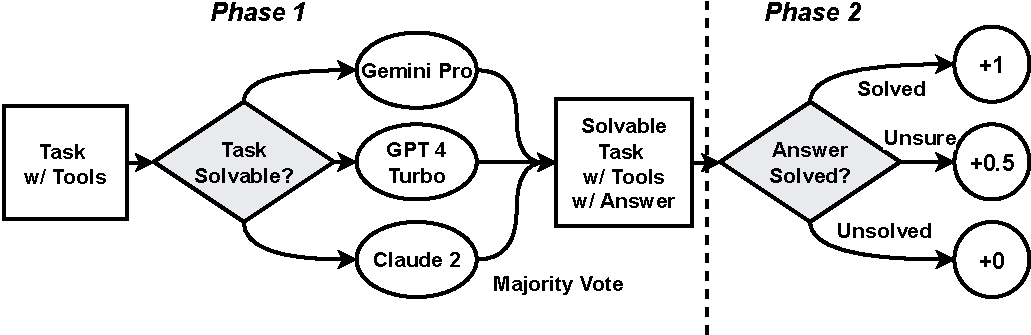
\includegraphics[width=\linewidth]{figs/SoPR.pdf}
    \caption{The process of our SoPR evaluation.}
    \label{fig:SoPR}
\end{figure}


\paragraph{API Calling Rules.}
Based on the caching system and the API simulator, we create API calling rules to ensure the stability of the virtual API server.
When a call request $(\mathrm{e},\mathrm{args})$, where $\mathrm{e}$ is the API endpoint and $\mathrm{args}$ is the arguments for that endpoint, is received, the system will first search the caching system for $(\mathrm{e},\mathrm{args})$ pair.
If a cache hit exists, the cached response will be directly returned.
When there is a cache miss, then the system will try to call the real API for a response to maintain the reality of the whole system.
If the real API calling is successful, the response will be returned.
However, when the caching system does not contain and the real API is not available, the system will finally call the simulated API. 
The final response whether from the real API or the simulated API will be saved to update in the caching system.
% Note that this will not affect the performance because all models evaluated will use the same response to a call whenever the the first call is made.

\subsection{Stable Evaluation System}
\label{sec:evaluation_system}

In this section, we propose a two-phase evaluation process, including judging solvable tasks and evaluating with two metrics, as shown in~\Cref{fig:SoPR}. Moreover, we replace all the automatic evaluators with \texttt{gpt-4-turbo}.

\paragraph{Judging Solvable Tasks.}\label{sec:judge_solvable_tasks}
\begin{table}[t!]
  \centering
  \small
  \resizebox{\linewidth}{!}{
  \begin{tabular}{lccccccc}
    \toprule
    & \textbf{I1-I} & \textbf{I1-C} & \textbf{I1-T} & \textbf{I2-I} & \textbf{I2-C} & \textbf{I3-I} & \textbf{Total}\\
    \midrule
    \textbf{Full} & 200 & 200 & 200 & 200 & 200 & 100 & 1,100 \\
    \textbf{Solvable} & 163 & 153 & 158 & 106 & 124 & 61 & 765\\
    % \midrule
    % \textbf{Total} & \multicolumn{2}{c}{765} & \multicolumn{3}{c}{1100} \\
    \bottomrule
  \end{tabular}}
  \caption{Statistics of original full and solvable tasks before and after judging. \texttt{C,I,T} stands for the Category, Instruction and Tool subgroup of the test set. Experiments below follow the denotation.}
  \label{tab:task_filteration}
\end{table}
Considering that both unsolvable and unsure tasks would introduce enormous randomness while the results of tasks fluctuate wildly, we try to obtain a fixed collection of solvable tasks to eliminate the problems.
To achieve this, we use three state-of-the-art LLMs, i.e., \texttt{gpt-4-turbo}, \texttt{gemini-pro}, and \texttt{claude-2}, to determine whether a task is solvable or unsolvable.
The prompt is shown in \Cref{app:prompt_task_solvability}.
The task will be judged as solvable when more than two models evaluate it as solvable.
The statistics of solvable tasks across all test datasets in ToolBench are shown in \Cref{tab:task_filteration}. 
% All reported scores are on the solvable tasks in the following experiment section.

\begin{table*}[t!]
    \centering
    \small
    \resizebox{\textwidth}{!}{
    \begin{tabular}{lccccccc}
        \toprule
        \textbf{Method} & \textbf{I1 Instruction} & \textbf{I1 Category} & \textbf{I1 Tool} & \textbf{I2 Category} & \textbf{I2 Instruction} & \textbf{I3 Instruction} & \textbf{Average} \\
        \midrule
     3.5 0613 (C)  & 52.2{\tiny $\pm{1.1}$} & 47.3{\tiny $\pm{0.6}$} & 53.6{\tiny $\pm{1.3}$} & 42.5{\tiny $\pm{2.1}$} & 35.8{\tiny $\pm{2.0}$} & 48.1{\tiny $\pm{0.8}$} & 46.6{\tiny $\pm{1.3}$} \\
    3.5 0613 (C)  & 60.3{\tiny $\pm{1.3}$} & 66.2{\tiny $\pm{1.2}$} & 67.1{\tiny $\pm{0.0}$} & 59.1{\tiny $\pm{0.4}$} & 51.3{\tiny $\pm{1.2}$} & 73.8{\tiny $\pm{2.3}$} & 63.0{\tiny $\pm{1.1}$} \\
    
    4 0613 (C) & 45.5{\tiny $\pm{0.4}$} & 57.4{\tiny $\pm{0.3}$} & 48.8{\tiny $\pm{0.7}$} & 43.0{\tiny $\pm{0.7}$} & 46.5{\tiny $\pm{0.9}$} & 48.1{\tiny $\pm{1.5}$} & 48.2{\tiny $\pm{0.8}$} \\
    4 0613 (D) & 57.3{\tiny $\pm{0.6}$} & 57.3{\tiny $\pm{0.3}$} & 60.9{\tiny $\pm{1.0}$} & 57.9{\tiny $\pm{1.0}$} & 51.3{\tiny $\pm{0.8}$} & 66.4{\tiny $\pm{2.4}$} & 58.5{\tiny $\pm{1.0}$} \\
    T-LLaMA (C) & 32.3{\tiny $\pm{1.0}$} & 40.3{\tiny $\pm{0.8}$} & 36.7{\tiny $\pm{0.5}$} & 34.7{\tiny $\pm{0.7}$} & 25.2{\tiny $\pm{0.4}$} & 33.9{\tiny $\pm{1.5}$} & 33.9{\tiny $\pm{0.8}$} \\
    T-LLaMA (D) & 44.5{\tiny $\pm{0.9}$} & 49.6{\tiny $\pm{1.3}$} & 48.9{\tiny $\pm{2.7}$} & 50.8{\tiny $\pm{1.1}$} & 31.9{\tiny $\pm{1.9}$} & 53.6{\tiny $\pm{2.0}$} & 46.6{\tiny $\pm{1.7}$} \\
    \midrule
   3.5 1106 (C)& 50.4{\tiny $\pm{0.5}$} & 45.1{\tiny $\pm{1.4}$} & 50.8{\tiny $\pm{0.3}$} & 48.7{\tiny $\pm{0.8}$} & 42.1{\tiny $\pm{0.4}$} & 55.7{\tiny $\pm{0.0}$} & 48.8{\tiny $\pm{0.6}$} \\
    3.5 1106 (D) & 62.8{\tiny $\pm{0.3}$} & 63.9{\tiny $\pm{1.2}$} & 65.6{\tiny $\pm{0.3}$} & 56.5{\tiny $\pm{0.7}$} & 56.9{\tiny $\pm{1.2}$} & 67.2{\tiny $\pm{1.3}$} & 62.2{\tiny $\pm{0.8}$} \\
    4 Turbo (C) & 52.8{\tiny $\pm{1.3}$} & 56.6{\tiny $\pm{0.9}$} & 51.9{\tiny $\pm{0.5}$} & 51.9{\tiny $\pm{1.0}$} & 52.8{\tiny $\pm{0.8}$} & 52.5{\tiny $\pm{0.0}$} & 53.1{\tiny $\pm{0.8}$} \\
    4 Turbo (D) & 59.2{\tiny $\pm{0.5}$} & 61.7{\tiny $\pm{0.7}$} & 65.7{\tiny $\pm{1.0}$} & 55.6{\tiny $\pm{0.6}$} & 55.2{\tiny $\pm{0.4}$} & 66.1{\tiny $\pm{4.3}$} & 60.6{\tiny $\pm{1.3}$} \\

         \bottomrule
    \end{tabular}
    }
    \caption{Solvable pass rate scores. We run all models once, evaluate three times and take the average results. ``3.5 0613'', ``4 0613'', ``3.5 1106'', ``4 Turbo'', ``T-LLaMA'' stands for \texttt{gpt-3.5-turbo-0613}, \texttt{gpt-4-0613}, \texttt{gpt-3.5-turbo-1106}, \texttt{gpt-4-turbo-preview}, 
    \texttt{ToolLLaMA v2} respectively. C and D stand for CoT and DFS respectively. The experiments below follow the denotation. We use \texttt{gpt-4-turbo-2024-04-09} as the evaluator. Evaluation done on May 2024.}
    \label{tab:main_sopr}
\end{table*}




    
% \begin{table}[h!]
%     \centering
%     \small
%     \begin{tabular}{lcc}
%         \toprule
%         \multirow{2}{*}{\textbf{Group}} & \textbf{After} & \textbf{Before} \\
%         & \textbf{Filtration} & \textbf{Filtration}\\
%         \midrule
%         {I1 Instruction} & 163 & 200\\
%         {I1 Category }& 153 & 200 \\
%         {I1 Tool} & 158 & 200 \\
%         {I2 Instruction} & 106 & 200\\
%         {I2 Category} & 124 & 200 \\
%         {I3 Instruction} & 61 & 100 \\
%         \midrule
%         {{Total}} & 765& 1100\\
%         \bottomrule
%     \end{tabular}
%     \caption{Query count statistics before and after filtration. \csj{todo}}
%     \label{tab:task_filteration}
% \end{table}

\paragraph{Metrics.}
We then report Solvable Pass Rate (SoPR) and Solvable Win Rate (SoWR) based on our obtained solvable tasks.
Due to the limitation of \texttt{gpt-3.5-turbo-16k} in tool learning, we uniformly adopt \texttt{gpt-4-turbo} as the automatic evaluator.
SoPR is in essence PR with all tasks solvable and only assesses the answers using the same prompt in ToolBench.
The evaluator assigns outcomes of answers categorised as Solved, Unsolved, or Unsure, which respectively contribute scores of 1, 0.5, and 0 to the overall SoPR calculation.
As for SoWR, when one is solved and the other is unsolved, the solved one wins.
Under other circumstances, \texttt{gpt-4-turbo} will be used to make a win-lose decision.  
% Note that the evaluation will be made whenever an \texttt{Unsure} label occurs.
% When calculating SoPR, the task description, available tools are fed into the automatic evaluator, using the same prompt as that in evaluating answer status when calculating Pass Rate\footnote{Prompts used to evaluate Pass Rate and Win Rate from ToolBench are at \url{https://github.com/OpenBMB/ToolBench/blob/master/toolbench/tooleval/evaluators/tooleval_gpt-3.5-turbo_default/template.txt}}.
% Furthermore, we improved the Win Rate with our SoPR to make it more stable, named Solvable Win Rate (SoWR). 
% Originally, when two methods received a \texttt{Passed} label and a \texttt{Failed} label during Pass Rate evaluations, the one with \texttt{Passed} label always wins when making Win Rate evaluations. Under other circumstances, an LLM based automatic evaluator will be used to make a win-lose decision. 




% \begin{table}[]
%     \centering
%     \small
%     \begin{tabular}{c|cc}
%         \toprule
%         \textbf{Methods} &  \\
%         \midrule
%          GPT 4 Turbo & 74.0 & 78.0\\
%          GPT 3.5 Turbo & 68.0 & 56.0 \\
%          \bottomrule
%     \end{tabular}
%     \caption{Human evaluation on answer solving (for pass rate) and comparison (for win rate).}
%     \label{tab:human_eval_task}
% \end{table}



\section{Experiment}

\subsection{Performance}\label{sec:performance}

% \textcolor{red}{Run different baseline models on the benchmark. The goal is to show that ranking of models on the benchmarks is the same as the precedents, i.e. improved stability will not change discrimination of the benchmark.}
Following ToolBench, we run \texttt{gpt-3.5-0613}, \texttt{gpt-4-0613}, \texttt{ToolLLaMA-v2} with CoT and DFS, replenishing with latest models \texttt{gpt-3.5-1106} and \texttt{gpt-4-turbo}.  
The results of SoPR and SoWR are shown in \Cref{tab:main_sopr,tab:main_sowr}. Generally, GPT-4 series models outperform GPT-3.5 models, while ToolLLaMA performs worst with the same inference algorithm.
Also, DFS significantly outperforms CoT whichever LLMs are used.
These phenomena are consistent with ToolBench.
Furthermore, probably thanks to the improved function calling capabilities, newer GPT models performed better. 
% Nevertheless, with more stable tools, gaps between LLMs are smaller with DFS than with CoT. This may indicate that more trials can significantly boost problem-solving performance.
\begin{table}[t!]
    \centering
    \small
    \resizebox{\linewidth}{!}{
    \begin{tabular}{lccccccc}
        \toprule
        \textbf{Method} & \textbf{I1-I} & \textbf{I1-C} & \textbf{I1-T} & \textbf{I2-I} & \textbf{I2-C} & \textbf{I3-I} & \textbf{Avg} \\
        \midrule
        3.5 0613 (D) & 60.7 & 67.3 & 59.5 & 63.2 & 62.1 & 75.4 & 64.7 \\
        4 0613 (C) & 54.6 & 58.8 & 58.2 &  75.5 & 60.5 & 62.3 & 61.7 \\
        4 0613 (D) & 62.6 & 62.7 & 58.2 & 74.5 &62.9 &  67.2 & 64.7 \\
        T-LLaMA (C) & 31.3 &28.1 &  33.5 & 35.8 & 33.9 &  24.6 & 31.2 \\
        T-LLaMA (D) & 44.8 & 45.8 & 44.3 & 59.4 & 41.1 & 50.8 & 47.7 \\
        \midrule
        3.5 1106 (C) &  47.2 & 47.7 & 44.9 & 50.9 & 54.0 & 62.3 & 51.2 \\
        3.5 1106 (D) & 55.8 &53.6 &  51.9 & 68.9 & 59.7 & 68.9 & 59.8 \\
        4 Turbo (C) & 71.2 &{77.1} &  61.4 & { 79.2} & {71.8} & {67.2} & {71.3} \\
        4 Turbo (D) & {73.0} &{75.2} &  {68.4} &  {77.4} & {66.9} & {60.7} & {70.2} \\
        \bottomrule
    \end{tabular}}
    \caption{Solvable Win Rate scores. We run all models once against \texttt{GPT-3.5-Turbo-0613 + CoT} and evaluate three times. We follow the ToolBench implementation to take the most frequent result for each query during evaluation. The experiments below follow the denotation. We use \texttt{gpt-4-turbo-2024-04-09} as the evaluator. Evaluation done on May 2024.}
    \label{tab:main_sowr}
\end{table}

\subsection{Stability of Virtual API Server}
% \textcolor{red}{Manually make ... of the APIs down (set probability of each calling APIs ), report the performance change of different methods. Aim to show the instability of the original system and stability of our system.} Results are shown in 
\begin{figure}[h!]
    \centering
    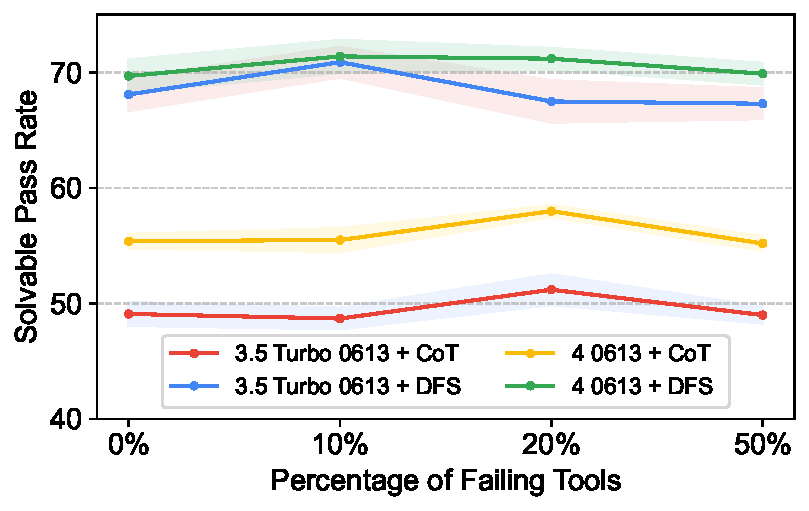
\includegraphics[width=\linewidth]{figs/virtual_solving_scores.pdf}
    \caption{Performance change when manually making APIs down with our virtual online API system. The results are averaged over all six groups. Solving rates are reported. We run each experiment one time and evaluate it three times and take the average score. Unless otherwise stated, \texttt{gpt-4-turbo-preview} at the time of testing is used in this section. This experiment was done in Feb 2024.}
    \label{fig:simulated_api_stability_test}
\end{figure}

Following the same setups as in \Cref{api_status}, we manually make the same success tools not available during the running time.
In our design, when a call is on an unavailable tool, it will be directed to the simulated API immediately.
Compared to \Cref{api_status}, the results as shown in \Cref{fig:simulated_api_stability_test} are much more stable with our virtual API server.
Even when 50\% of APIs are not available, changes in performance are still not significant, which is explainable within the range of variance.



% \textcolor{red}{change gpt-4 versions and other hyperparameters and run multiple sets of experiments. Aim to show change of GPT-4 won't affect the stability significantly.} 
Considering we use \texttt{gpt-4-turbo} as the backbone of the API simulator which may change even with the same version number, we ablate different versions and different temperatures of \texttt{gpt-4-turbo}.
The results are shown in \Cref{tab:server_config}.
Under different settings of the backbone LLMs, the performance change is still acceptable within the variance of LLM evaluation, indicating the robustness of our API simulators.



% \textcolor{red}{Discussion: An ultimate solution is to train a open-source models that make mock the API behavior well.
% }




% \begin{figure}
%     \centering
%     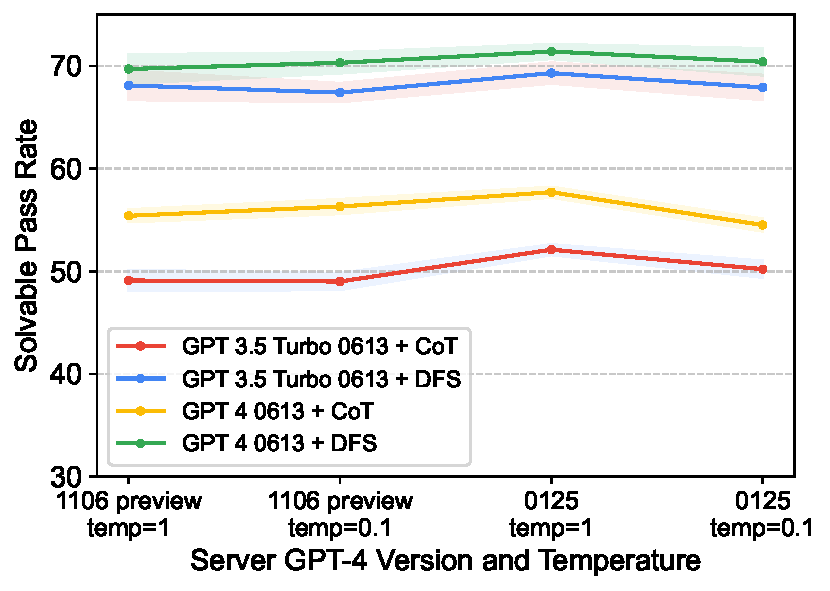
\includegraphics[width=\linewidth]{figs/virtual_solving_scores_against_server.pdf}
%     \caption{Performance of baselines with different settings of the LLM server. The results are averaged over all six groups. Solving rates are reported. We run each experiment one time and evaluate three times and take the average score.}
%     \label{fig:server_config}
% \end{figure}

\begin{table}
    \centering
    \small
    \resizebox{\linewidth}{!}{

    \begin{tabular}{lcccc}
        \toprule
        \multirow{2}{*}{\textbf{GPT-4 Config}} & \multicolumn{2}{c}{\textbf{1106-preview}} &  \multicolumn{2}{c}{\textbf{0125}} \\
        & \texttt{T=1} & \texttt{T=0.1} & \texttt{T=1} & \texttt{T=0.1}\\
        \midrule
         3.5 0613 (C) & 49.1{\tiny $\pm{1.0}$}  & 49.0{\tiny $\pm{0.8}$} & 52.1{\tiny $\pm{0.5}$} & 50.2{\tiny $\pm{0.8}$} \\
         3.5 0613 (D) & 68.1{\tiny $\pm{1.4}$}  & 67.4{\tiny $\pm{0.9}$} & 69.3{\tiny $\pm{1.0}$} & 67.9{\tiny $\pm{1.2}$}\\
         4 0613 (C) & 55.4{\tiny $\pm{0.6}$}  & 56.3{\tiny $\pm{0.7}$} & 57.7{\tiny $\pm{0.5}$} & 54.5{\tiny $\pm{0.6}$} \\
         4 0613 (D) & 69.7{\tiny $\pm{1.4}$}  & 70.3{\tiny $\pm{1.0}$} & 71.4{\tiny $\pm{0.7}$} & 70.4{\tiny $\pm{1.3}$}\\
         \midrule
         3.5 1106 (C) & 52.1{\tiny $\pm{0.7}$}  & 51.1{\tiny $\pm{0.5}$} & 54.5{\tiny $\pm{0.9}$} & 52.7{\tiny $\pm{0.6}$} \\
         3.5 1106 (D)  & 69.9{\tiny $\pm{0.7}$}  & 71.2{\tiny $\pm{0.9}$} & 70.0{\tiny $\pm{0.9}$} & 71.0{\tiny $\pm{0.9}$}\\
         4 Turbo (C) & 60.8{\tiny $\pm{0.7}$}  & 62.4{\tiny $\pm{0.8}$} & 63.6{\tiny $\pm{0.4}$} & 64.0{\tiny $\pm{1.1}$} \\
         4 Turbo (D) & 73.2{\tiny $\pm{1.1}$}  & 76.2{\tiny $\pm{0.9}$} & 75.0{\tiny $\pm{0.7}$} & 77.3{\tiny $\pm{0.9}$}\\     
        \bottomrule
    \end{tabular}
    }
    \caption{Performance of baselines with different settings of the LLM server. Results are averaged over all groups and reported in SoPR. We run each experiment one time and evaluate three times and take the average score.}
    \label{tab:server_config}
\end{table}

% Different models, same input, same outputs, temp=0




\subsection{Turing Test of API Simulator}
% \textcolor{red}{Aiming at testing the reality of APIs. 
% Sampling 100 API calls from real API responses and LLM faked responses, and ask GPT-4 / Human whether the two are indistinguishable (guess which is model and which is real). If the results are around 50\%. Then the test is passed.}
To test the effectiveness of API simulators, we design a ``Turing Test''~\cite{Turing2009} between the real APIs and the simulated ones.
% To successfully run experiments on a tool-learning benchmark, the fundamental requirement for the API system is that the responses of the API system are usable and believable by the testing model. 
% In this way, the testing model can use the outputs to finish an instruction. 
Note that we believe it is not required for API simulators to exactly output the same answers as those of real APIs, where rationality is more important.
% This is because the exact reality of API responses is not required for task completion.
For example, when a query asks about the weather today, the API simulator does not need to retrieve the ``real'' temperature. Instead, the API simulator needs to generate a reasonable temperature number.

To do the test, we first sample 70 available real APIs and their corresponding simulated APIs. 
% We then manually filter out unsuccessful real API calls, resulting in 70 API calls.
Given the API callings and their real and simulated response pairs, we ask three human annotators to determine which response more closely resembles an actual API response overall, based on the given descriptions of the API functions.
We ask human annotators to evaluate along three dimensions: Overall, Format Accuracy and Answer Relevance.
The annotator first need to answer which response is overall more like a real response.
When assessing format accuracy, annotators must determine which response more accurately adheres to the format specifications outlined in the documentation. In evaluating answer relevance, they are tasked with identifying which response more effectively fulfills the instruction in accordance with the documentation's guidelines.
The results are shown in ~\Cref{fig:turing_test}.
Surprisingly, human annotators cannot distinguish simulated and real APIs very well, where the simulated APIs are judged to act more like real situations.
Moreover, the proportion of tie is much larger, indicating that simulated APIs can work very similarly to real APIs.
% To further analyze the reason, we further ask human annotators to distinguish two kinds of APIs in terms of format accuracy and answer relevance only. As shown in \Cref{fig:turing_test}, one can see simulated APIs can work very similarly to the real APIs.


% \begin{table*}
%     \centering
%     \small
%     \begin{tabular}{cccccccccc}
%         \toprule
%         & \multicolumn{3}{c}{\textbf{Overall}} & \multicolumn{3}{c}{\textbf{Format Accuracy}}& \multicolumn{3}{c}{\textbf{Answer Relevance}}\\
%         \cmidrule(lr){2-4}
%         \cmidrule(lr){5-7}
%         \cmidrule(lr){8-10}
%         & {Real} &  {Simulated} & {Tie} & {Real} &  {Simulated} & {Tie}& {Real} &  {Simulated} & {Tie} \\
%         \midrule
%         % GPT-4-Turbo & 31.0 & 62.1 & 6.9 & 34.5 & 58.6 & 6.9 & 37.9 & 55.2 & 6.9  \\
%         % Gemini Pro & 31.0 & 69.0 & 0.0 & 20.7 & 79.3 & 0.0 & 31.0 & 65.5 & 3.4 \\
%         Human & 12.9\% & 20\% & 67.1\% & 0 \% & 5.7\% & 94.3\% & 10\% & 20\% & 70\% \\
%         \bottomrule
%     \end{tabular}
%     \caption{Results of the ``Turing Test'' for the real and LLM simulated APIs. \textcolor{red}{TODO: Change to bar figure.}}
%     \label{tab:turing_test}
% \end{table*}

\begin{figure}[t!]
    \centering
    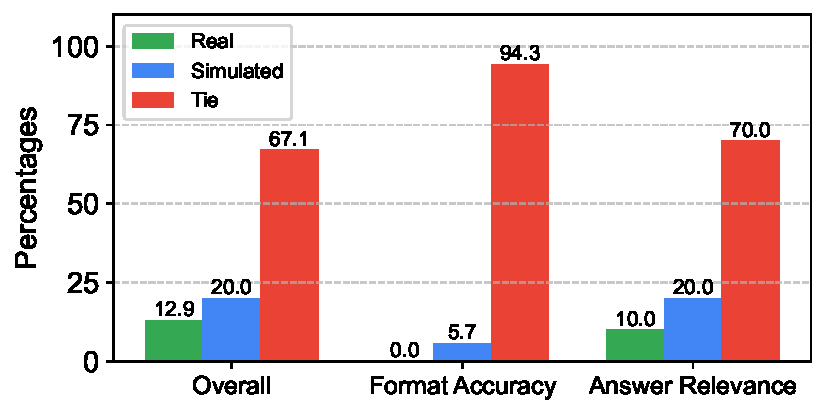
\includegraphics[width=\linewidth]{figs/turing_test.pdf}
    \caption{Results of the ``Turing Test'' for the real and simulated APIs. Results are win-lose-tie percentages.}
    \label{fig:turing_test}
\end{figure}

% We sample 50 LLM simulations from the Turing Test questions discussed in Section 4.3. Then we invite a human evaluator to answer whether the LLM simulation follows the documentation, i.e., whether it is a reasonable simulation that obeys the setting of the documentation. Results show that 90% of the simulations are deemed to be reasonable, 6% are not reasonable and 4% are not sure. It shows that the simulated APIs can well follow documentation.


In addition to the Turing Test mentioned above, we assess the quality of LLM simulations by evaluating the adherence of simulated outputs to their corresponding documentation. To conduct this evaluation, we randomly sample 50 simulated outputs along with their documentation from the Turing Test dataset. A human evaluator is then tasked with determining whether the LLM simulations reasonably follow the provided documentation. The results indicate that 90\% of the simulations are deemed reasonable, 6\% are considered unreasonable, and 4\% are uncertain. These findings suggest that the LLM is highly capable of generating simulated responses that adhere closely to the provided documentation.

% \begin{itemize}
%     \item Different inputs -> different outputs, same formats
% \end{itemize}


\subsection{Diversity of API Simulator}
% \textcolor{red}{Aim to show that API calls are diverse enough, so that the effective numbers of APIs won't decrease with simulated APIs.}
% \begin{enumerate}
%     \item Select a category of APIs, call these APIs in real and simulated ways. Calculate embeddings of these calls and see clustering outputs.
%     \item Call a selected APIs (potentially 10) with various arguments. See the difference across different arguments for both real and simulated APIs.
% \end{enumerate}
With the LLM simulation, API simulators will not exactly feedback the same as real APIs. 
Hence, a natural concern is whether the simulated APIs will degrade in diversity in API functionalities.
To study the problem, firstly, we explore the distribution of real and simulated API responses.
We first use all 246 APIs in the \texttt{Tool} API category from the successful APIs mentioned in \Cref{api_status}.
Then, we use the same call arguments to call these real and simulated APIs.
All the responses are encoded using S-BERT~\cite{reimers-2019-sentence-bert} and their corresponding embeddings are visualised by UMAP~\cite{mcinnes2018umap-software}. 
Detailed configuration is shown in \Cref{app:diversity_conf}.
The result is shown in \Cref{fig:diversity_comparison}. As can be seen from the figure, real and simulated APIs occupied similar embedding space, indicating that the diversity of simulated APIs is similar to the real APIs.

\begin{figure}[h!]
    \centering
    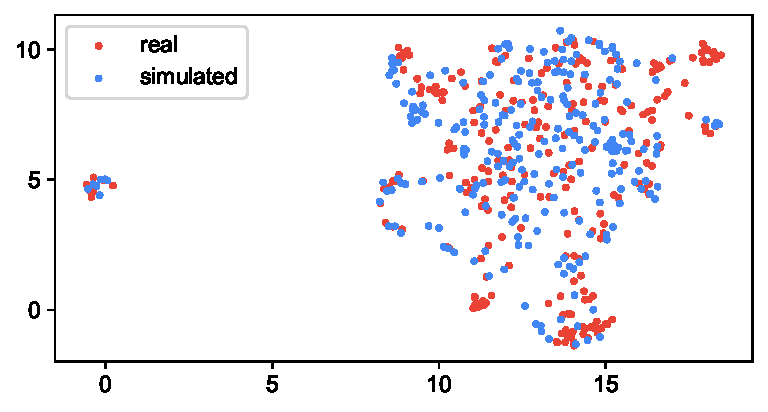
\includegraphics[width=\linewidth]{figs/diversity_comparison.pdf}
    \caption{Visualisation of the embeddings of responses from real and simulated APIs.}
    \label{fig:diversity_comparison}
\end{figure}

Secondly, we try to explore the behaviour when a simulated API is given several calls with different input arguments. 
We sample 60 APIs from all successful APIs and make 5 different calls to each API, using the same prompt as in \Cref{app:prompt_make_call}.
We then count the number of APIs that give exactly the same responses in any 2 of the 5 calls. Results show that only 2 of 60 APIs contain such responses, which supports the sufficient diversity of our simulated APIs.


\subsection{Effectiveness of Caching System}
% We run experiments on different methods and record the cache hit rate.
To show the effectiveness of our caching system in maintaining the stability of the virtual API server, we run several methods and record the cache hit rates. In detail, we run four methods used in ToolBench, \texttt{gpt-3.5-turbo-0613} and \texttt{gpt-4-0613} with CoT and DFS. Reproduction data in ToolBench of these methods has been used in the cache. Results are recorded in~\Cref{tab:cache_hit}, which shows that rerunning these in-domain methods has a very high cache hit rate. This means that most of the call responses are fixed and instability from the API system are much smaller. Nevertheless, models and methods may change over time, and therefore, we further run \texttt{gpt-3.5-turbo-1106} and \texttt{gpt-4-turbo-preview} with CoT and DFS.  As can be seen in the table, although the cache hit rates are smaller with these out-of-domain methods, the scores are still high enough to mitigate the instability significantly.



\subsection{Human Evaluation of Evaluator}
\label{sec:evaluator}

Considering that GPT-3.5 is limited to evaluating the performance in tool learning, we replace the automatic evaluators with stronger LLMs.
In this section, we manually assess the correctness of different automatic evaluators. 
Here, we sample 100 task-solvable questions, 50 answer-solving questions in the PR / SoPR evaluation, and 50 comparison questions in the WR / SoWR evaluation from the experiments running.

\begin{table}
    \centering
    \small
    \begin{tabular}{lccc}
        \toprule
        \textbf{Methods} & \textbf{Final} & \textbf{Mid} & \textbf{Start}\\
        \midrule
        GPT 3.5 Turbo 0613 + CoT & 96.7 & 36.2 & 11.7 \\
        GPT 3.5 Turbo 0613 + DFS & 97.0 & 34.5 & 11.6 \\
        GPT 4 0613 + CoT &  96.5 & 36.2 & 11.7\\
        GPT 4 0613  + DFS & 97.0 & 35.0 & 11.7 \\
         \midrule 
        GPT 3.5 Turbo 1106 + CoT & 91.4 & 35.1 & 11.8\\
         GPT 3.5 Turbo 1106 + DFS & 75.8 & 34.5 & 11.4 \\
        GPT 4 Turbo + CoT & 88.2 & 35.0 & 11.6 \\
        GPT 4 Turbo + DFS & 77.8 & 34.5 & 11.8\\
        \bottomrule
    \end{tabular}
    \caption{Cache hit rate (\%) with various models and methods. Final, Mid, and Start represent the final version of the cache, the mid-way version containing 151,152 (91.6\%) items of the final version, and the starting version containing only the train and test set. Experiments are independent runs of \Cref{sec:performance} with fixed cache, run on 13 Feb 2024.}
    \label{tab:cache_hit}
\end{table}
We then collect all the corresponding answers of different LLMs during previous evaluations.
% We use the same prompt and format as in the experiments. 
% We run \texttt{gpt-3.5-turbo}, \texttt{gpt-4-turbo}, \texttt{gemini-pro}, and \texttt{claude-2} on task solvable questions and \texttt{gpt-3.5-turbo}, \texttt{gpt-4-turbo} on answer solving and comparison questions.
These questions are further manually labeled by three human annotators to obtain the ground truth.
With the ground truth, we calculate the accuracy scores of these models and show the results in \Cref{tab:human_eval_task}. 
It can be seen that our used LLMs (i.e., Claude 2, Gemini, and GPT-4) are much better than GPT-3.5 in ToolBench to determine the solvability of tasks, where the Gemini and GPT-4 outperform by a large margin.
In both the evaluation of answers and comparison, GPT-4 significantly outperforms GPT-3.5, especially in the comparison to compute WR.
It is worth noting that all the accuracies of GPT-3.5 are lower than 70\%, indicating that GPT-3.5 cannot assess the performance in tool learning.
% \texttt{gemini-pro} and \texttt{claude-2} perform much better than \texttt{gpt-3.5-turbo} as well, which supports our model choices when judging task solvability above. 
% As a result, we replace {gpt-3.5-turbo} with \texttt{gpt-4-turbo} in the experiments below.



% \begin{table*}[]
%     \centering
%     \small
%     \begin{tabular}{cccccccc}
%         \toprule
%         \textbf{Method} &G1 Cat & G1 Inst & G1 Tool & G2 Cat & G2 Inst & G3 Inst & Avg \\
%         \midrule
%          ChatGPT + CoT & \\
%          ChatGPT + DFS \\
%          GPT-4 + CoT \\
%          GPT-4 + DFS \\
%          ToolLLaMA + CoT \\
%          ToolLLaMA + DFS \\
%          \bottomrule
%     \end{tabular}
%     \caption{NLI score}
%     \label{tab:my_label}
% \end{table*}




% \subsection{Human Evaluation on the NLI Metric}